% Ella-Lovise  is writing

\subsection*{Problem 2.4}
\addcontentsline{toc}{subsection}{Problem 2.4}

\subsubsection*{Calculate sideslip angle}
\addcontentsline{toc}{subsubsection}{Calculate sideslip angle}

The sideslip angle is the angle from $x_b$ axis of {b} to the velocity vector of the vehicle, with positive rotation around the $z_b$ axis of {b} as given by the right-hand screw convention. The formula for sideslip is therefore:

\begin{equation}
    \boldsymbol{\beta}_r = \arcsin( v^b_r/U^b_r)
    \label{eq:beta_r}
\end{equation}

defined by the relative velocity $v_r$, from $\mathbf{V_r} = [u_r,v_r,w_r]^\top$, and relative speed $U_r$. The relative velocity in body frame in this assignment is defined by equation \eqref{eq:v_r}.The crab angle is defined in body, according to Fossen. In this assignment the relative velocity was defined to $\mathbf{v}^b_{b/n} = [1.5, 0,0]$, from problem 2.1. In problem 2.1 there was no current, and following the convention from problem 2.2, the velocity on a straight line relative to the ocean is given as $\mathbf{v}^b_{b/c} = [1.5, 0,0]$. \todo{åpen for omformuleirnger her ! } 

The sideslip angle was calculated using equation \eqref{eq:beta_r}, giving $0 ^\circ$. This result is as expected, since the relative velocity consists of $v=0$, and  $\mathbf{v}^b_{b/c} = [1.5, 0,0]$.  Because sideslip angle is defined by the relative velocities, and the vehicle tries to stick to a straight line, in reality the current will inflict a force upon the vehicle in a manner that will change the slope of the straight line, since the current is constant .  a   The result of the current carrying the vehicle will be noticeable on the crab angle, as discussed in later sections. 

\subsubsection*{Simulation of translational motion of the vehicle }
\addcontentsline{toc}{subsubsection}{Simulation of translational motion of the vehicle}

The simulation of the translational motion was performed using \texttt{MATLAB}. The initial conditions were $\phi = 0^\circ$, $\theta = 0^\circ$ and $\psi = 30^circ$ and start position at $\mathbf{0}$. With no current, $\mathbf{v}^b_{b/c} = \mathbf{v}^b_{b/n}$. To simulate the translational motion without current, the velocity of the vehicle relative to the ned was first calculated:
\begin{equation}
    \mathbf{v}^n_{b/n} = \mathbf{R}^n_b \mathbf{v}^b_{b/n} = \mathbf{R}^n_b [U \cos(\omega t), U \sin(\omega t), 0]^\top
    \label{eq:v_n_b_c}
\end{equation}


The position of the vehicle was found using Euler integration, meaning the position of vehicle is $\mathbf{p}\text{(i+1)}^n_{b} = \mathbf{p}(i)^n_{b} + \mathbf{v}(i)^n_{b/n}*h $, with timestep $h = 0.1$ and i equal the number of the iteration.
 
The  plotting of the translational motion with current, was also chosen to be in NED reference frame with the position relative to the NED, meaning $\mathbf{p}^n_{b}$. The first step was to calculate the velocity of the vehicle $\mathbf{v}^n_{b/c}$, as done in \eqref{eq:v_n_b_c}. Furthermore the velocity of the current relative to NED expressed in NED reference frame, $\mathbf{v}^n_{c/n}$ ,was calculated from equation \eqref{eq:v_n_c}. The expression for the velocity of the vehicle relative to NED  in NED reference frame is:


\begin{equation}
    \mathbf{v}^n_{b/n} = \mathbf{v}^n_{b/c} + \mathbf{v}^n_{c/n} = \mathbf{R}^n_b \mathbf{v}^b_{b/c} + \mathbf{v}^{n}_{c/n} 
    \label{eq:v_b_r}
\end{equation}

The expression for the position of the vehicle relative to NED reference frame is found by Euler integration, meaning $\mathbf{p}\text{(i+1)}^n_{b} = \mathbf{p}(i)^n_{b} + \mathbf{v}(i)^n_{b/n}*h $. The method used is the same as for the simulation without current.


The crab, course  and sideslip angle was calculated using respectively equation \eqref{eq:beta_2}, \eqref{eq:chi} and \eqref{eq:beta_r}, respectively. With $\mathbf{v}_r = \mathbf{v}^n_{b/c}$.  Because the arcsin command in \texttt{MATLAB}, \texttt{asin} only provides the angle between $-\frac{\pi}{2}$ and $\frac{\pi}{2}$,the crab angle and sideslip is approximated using atain2. This approximation is based on the assumption $w= 0$ and gives:

\begin{equation}
\begin{aligned}
	& \beta = atan2(v^b_{b/n}, u^b_{b/n} ) \\
	& \beta_r = atan2(v^b_{b/c}, u^b_{b/c} )  \\
	\label{eq:crab_slip_approx}
\end{aligned}
\end{equation}

\subsubsection*{Result after simulation}
\addcontentsline{toc}{subsubsection}{Result after simulation}

In \ref{fig:4_pos} the position of the vehicle relative to the NED is plotted using reference frame NED. Without current the vehicle makes a perfect circle with radius 100 m, as required and expected. With current the vehicle tries to make a perfect circle, but the current carries the vehicle in north-east direction, making the path to the vehicle relative to the ocean look like a spiral.

\begin{figure}[!ht] 
	\centering
	\begin{subfigure}[b]{0.45\textwidth}
		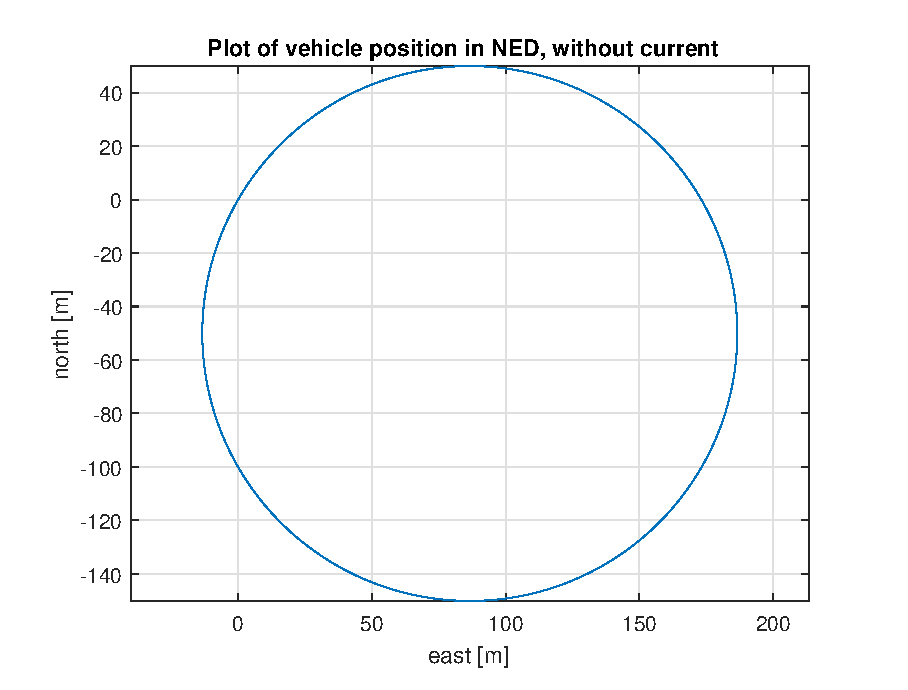
\includegraphics[width=\textwidth]{figures/4_pos.eps}
		\caption{Without current}
		%\label{fig:4_pos}
	\end{subfigure}
	~ %add desired spacing between images, e. g. ~, \quad, \qquad, \hfill etc. 
	%(or a blank line to force the subfigure onto a new line)
	\begin{subfigure}[b]{0.45\textwidth}
		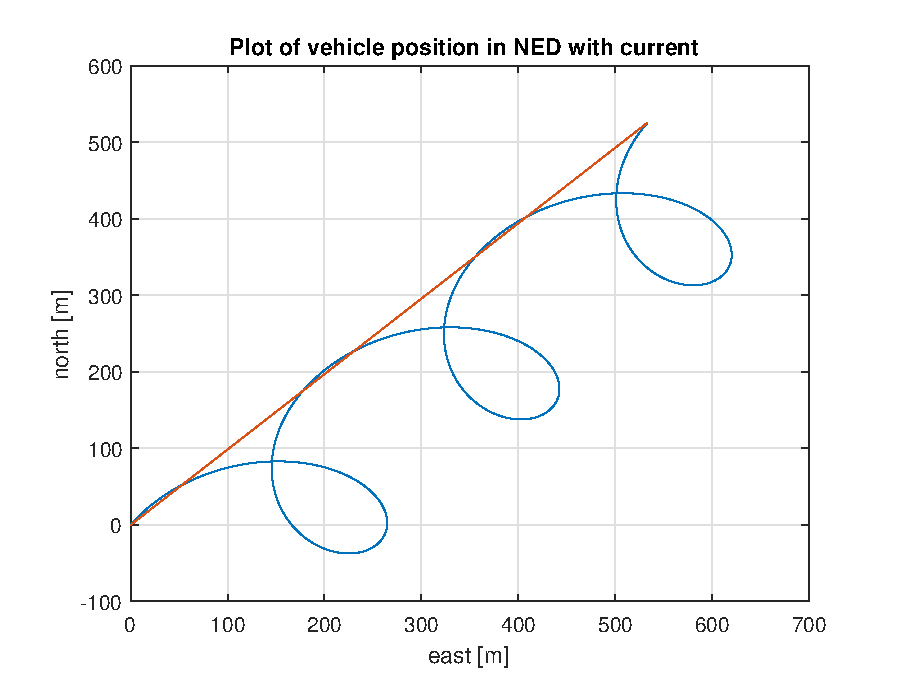
\includegraphics[width=\textwidth]{figures/4_pos_current}
		\caption{With current. The red line marks the flow of the current, the blue the position of the vehicle}
		\label{fig:4_pos_current}
	\end{subfigure}
	\caption{The position of the vehicle in reference frame NED}
	\label{fig:4_pos}
\end{figure}

The relative velocities will be the same with and without current. The vehicles velocity in body frame relative to current is defined ad $\mathbf{v}^b_{b/c} = [U \cos(\omega  *t), U \sin(\omega*t) , 0]$ and hence will not depend on current, $\omega$ is constant. This is shown in figure \figref{fig:4_vel}, which demonstrates the velocity of vehicle relative to the ocean current in NED reference frame. The plot in \figref{fig:4_vel} a) shows constant speed, since $\mathbf{v}^b_{b/c}$ consists of a cosine and sinusoidal  depending on both frequency and time. 

A plot of velocity  $\mathbf{v}^n_{b/n}$ affected by current is shown in figure \figref{fig:4_vel} b) . Since there is current   looking at the velocity of the body relative to NED, both the speed and velocity is  affected by the current. Because the relative velocity is $\mathbf{v}_r = v + v_c$, and $\mathbf{v}_c != \mathbf{0}$, the speed is not constant, but varies sinusoidal. The same goes for the velocity $\mathbf{v}^n_{b/n}$, affected by the constant current velocities. The reason for  $\mathbf{v}^n_{b/n}$ being periodically is that both the current and the relative velocity of the vehicle is periodic.

\begin{figure}[!ht]
	\centering
	\begin{subfigure}[b]{0.45\textwidth}
		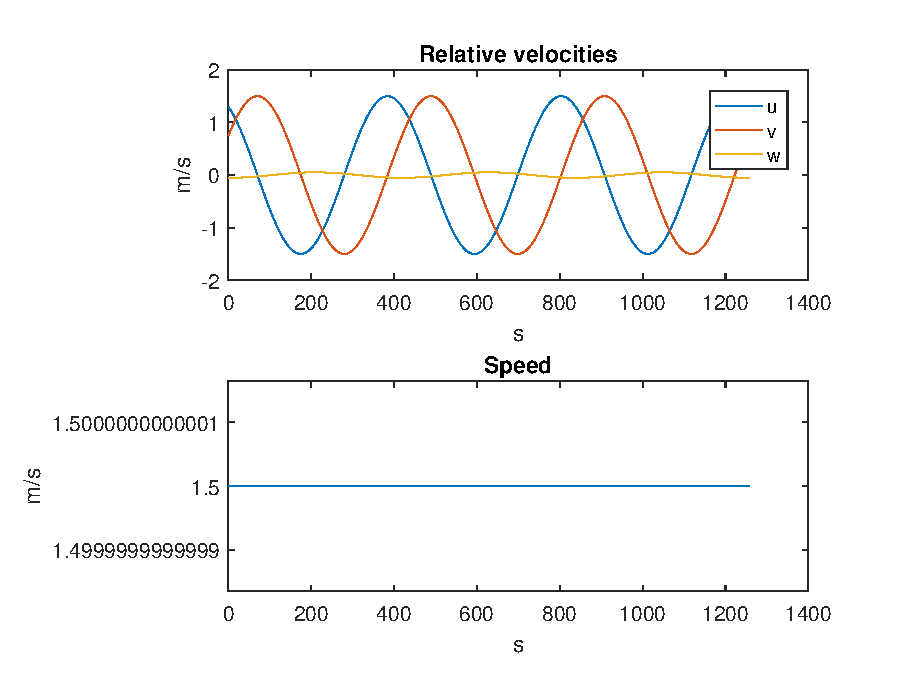
\includegraphics[width=\textwidth]{figures/4_vel}
		\caption{Without current}
		%\label{fig:4_vel}
	\end{subfigure}
	~ %add desired spacing between images, e. g. ~, \quad, \qquad, \hfill etc. 
	%(or a blank line to force the subfigure onto a new line)
	\begin{subfigure}[b]{0.45\textwidth}
		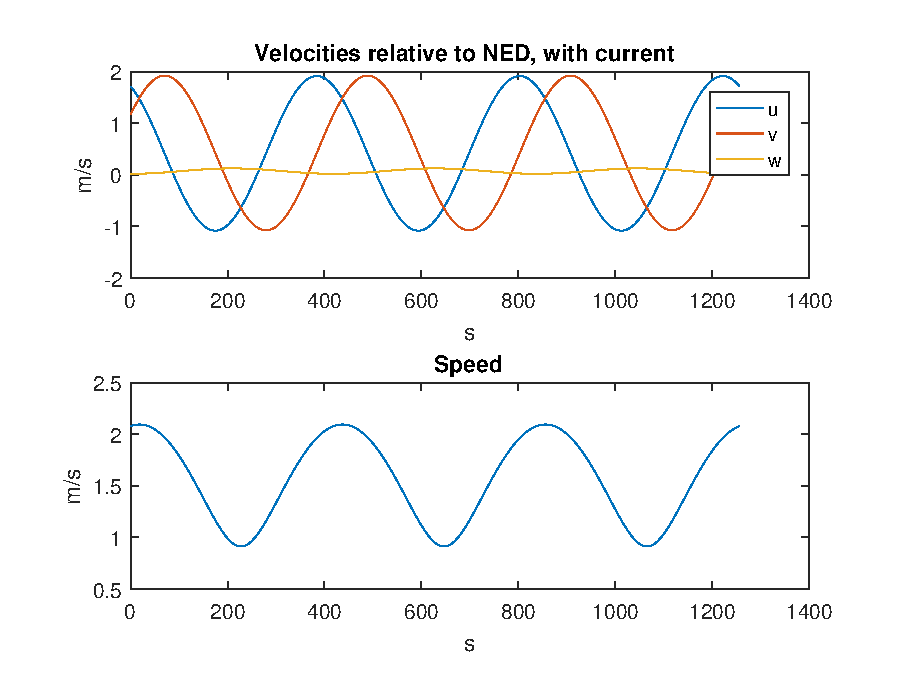
\includegraphics[width=\textwidth]{figures/4_vel_ned_with_cur}
		\caption{With current}
		%\label{fig:4_vel_ned_with_cur}
	\end{subfigure}
	\caption{The relative velocity and speed of the vehicle, defined equation \eqref{eq:v_n_r} in reference frame NED}
	\label{fig:4_vel}
\end{figure}


The plots of crab, sideslip and course angle is in figure \ref{fig:4_crab}. Crab, sideslip and course angle goes from $0-360^\circ$, all plots in this report restricted angles to stay within 0-360 degrees. It is reasonable that  the anlges goes from $0-360^\circ$ since the vehicle is driving in a circle with the bow  in the same direction. In the plot without current $\mathbf{v}^b_{b/c} = \mathbf{v}^b_{b/n} $, this means $\beta_r = \beta$, which is also clear from the plot. In the plot with current the sideslip angle $\beta_r$ is the same as in plot without current. The crab angle and course angle which depends upon the velocity of the current is therefore different in the plot with current. Since there is current, the relationship between $u^b$ and $v^b$ varies periodically, meaning the crab and course angle varies periodically. The reason for this is that the course angle  is linearly dependent upon crab angle and yaw. 

\begin{figure}[!ht]
	\centering
	\begin{subfigure}[b]{0.45\textwidth}
		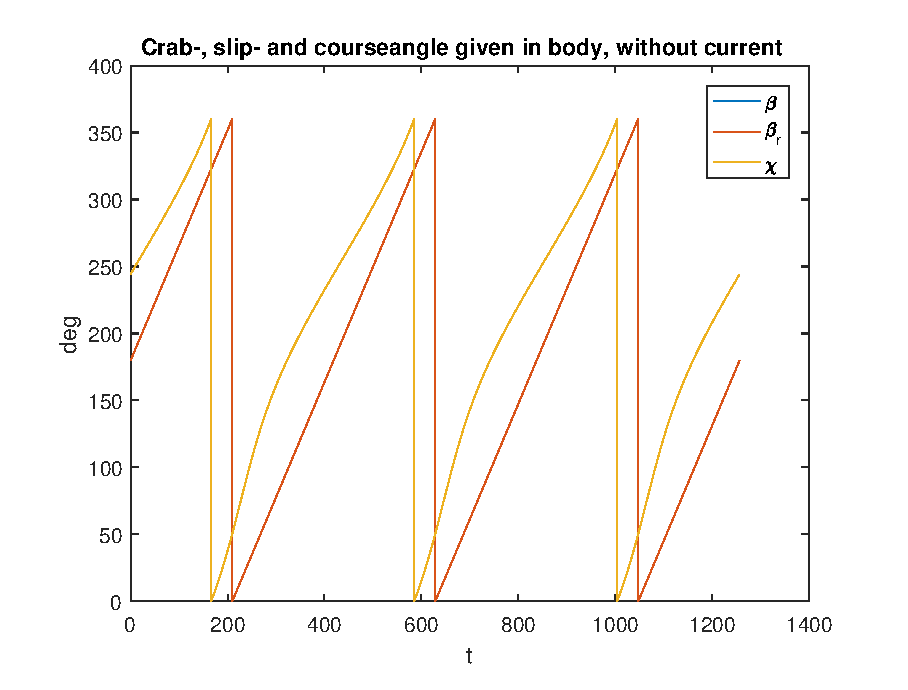
\includegraphics[width=\textwidth]{figures/4_crab_slip_course}
		\caption{Without current}
		%\label{fig:4_vel}
	\end{subfigure}
	~ %add desired spacing between images, e. g. ~, \quad, \qquad, \hfill etc. 
	%(or a blank line to force the subfigure onto a new line)
	\begin{subfigure}[b]{0.45\textwidth}
		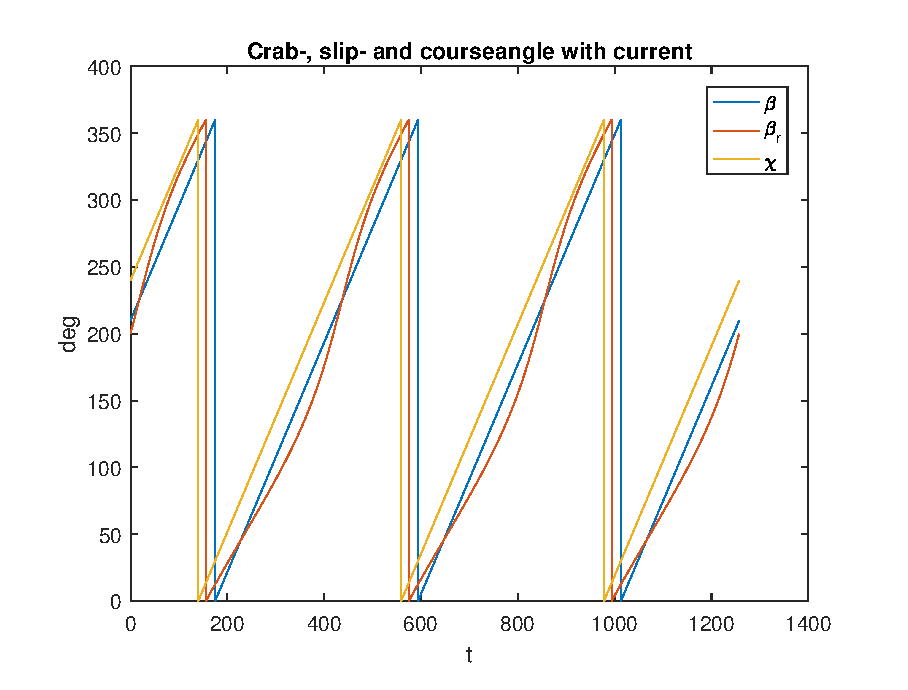
\includegraphics[width=\textwidth]{figures/4_crab_slip_course_current}
		\caption{With current}
		%\label{fig:4_vel_current}
	\end{subfigure}
	\label{fig:4_crab}
	\caption{The crab-, course and sidslip angles in reference frame NED}
\end{figure}

\subsection*{Problem 2.5}
\addcontentsline{toc}{subsection}{Problem 2.5}

The vehicle's turning rates are now assumed to be modeled by the Nomoto model and are:
\begin{equation}
	\frac{r}{\delta} (s) = \frac{K}{Ts+1}
\end{equation}

with $\delta$ equal the rudder angle, $K =0.1 s^{-1}$ and $T = 50s$.

The pitch and roll motions are given as
\begin{equation}
\begin{aligned}
	&\dot{p} + 2\zeta_p\omega_p p + \omega_p^2 \phi = 0\\
	&\dot{q} + 2\zeta_q\omega_q q + \omega_q^2 \theta = 0
	\label{eq:p_q_dot}
\end{aligned}
\end{equation}
with damping factors and natural frequencies as $\zeta_p = 0.1 $, $\zeta_q = 0.2 $, $\omega_p = 0.1 $ and $\omega_q = 0.05 $. 

\subsubsection*{Calculations of steady state}
\addcontentsline{toc}{subsection}{Problem 2.4}

The steady state angular velocities $p_s$, $q_s$ and $r_s$ during turning for a constant rudder angle $\delta$ may be found by setting $\dot{p}= \dot{q} = \dot{r} = 0$. The equation for $\dot{r}$ may be found by applying the inverse Laplace using the Nomoto equation. In \cite{Fossen2011} the time representation of the first order Nomotos model, equation (7.52) in \cite{Fossen2011} is estimated as 

\begin{equation}
    T\ddot{\psi} + \dot{\psi} = K \delta
    \label{eq:nomo_first_order_time}
\end{equation}

In this problem $\theta = 2.0 ^\circ$ and $\phi = 0.0 ^\circ$, giving $\dot{\psi}$ as approximately $r$. Using \eqref{eq:nomo_first_order_time} the  first order Nomoto-model time representation is given as:

\begin{equation}
    \dot{r} = - \frac{r}{T} +  \frac{K}{T} \delta
    \label{eq:r_time}
\end{equation}

Using \eqref{eq:r_time} and \eqref{eq:p_q_dot} and setting $\dot{p} =\dot{q} = \dot{r}$ this gives the following expression for the steady state of the angular  velocities:

\begin{equation}
\begin{aligned}
	& p_s = \frac{\omega_p^2 \phi}{ 2\zeta_p\omega_p} = \frac{1}{2} \phi \\
	& q_s = \frac{\omega_q^2 \theta}{2\zeta_q\omega_q} = \frac{1}{8} \phi \\
	& r_s = K \delta
	\label{eq:p_q_dot}
\end{aligned}
\end{equation}

This means the steady state angular velocities $p_s = \frac{1}{2} \phi ^\circ s^{-1}$, $q_s = \frac{1}{9} \theta ^\circ s^{-1}$, $r_s = 0.1 \delta ^\circ s^{-1}$. 

\subsection*{Problem 2.6}
\addcontentsline{toc}{subsection}{Problem 2.6}

In this problem the model of the vehicle is implemented by varying $\boldsymbol{\omega}^b_{b/n}$, described in equation \eqref{eq:r_time} and \eqref{eq:p_q_dot}. The system have the initial positions $\boldsymbol{\Theta} = [-1.0^\circ, 2,0^\circ, 0.0^\circ]^\top$ and $\boldsymbol{\omega}^b_{b/n} = [0,0,0]^\top s^{-1}$ . The start position is $\mathbf{p}^n_{b/n} = [0,0,0]^\top m$. The vehicle is still exposed to the current described in equation \eqref{eq:v_n_c}  and the rudder changes after 700 seconds from $\delta = 5^\circ$ to $\delta = 10^\circ$.

Since the current is constant in NED reference frame, the rotation of $\omega^n_{c/b} $ is zero, implying $\boldsymbol{\omega}^b_{c/b} = 0$. This means $ \boldsymbol{\omega}^b_{b/n} = \boldsymbol{\omega}^b_{b/c} + \boldsymbol{\omega}^b_{c/n}  = \boldsymbol{\omega}^b_{b/c} $. \todo{Should i be more spesific, or more wage ? What do you think Alexandra ?}

\subsection*{The code for simulation}
\addcontentsline{toc}{subsection}{The code for simulation}

The system is simulated in the file {\color{blue} attitude4.m}. The files start by initializing all the relevant variables. In the simulation the time step is $h = 0.1$ .

Because of varying $\boldsymbol{\omega}^b_{b/n}$, the Euler angles will change during the simulation. Consequently, the first thing to do for each iteration is to calculate the new rotation matrix $\mathbf{R}^n_b$, dependent on the current Euler angles. To find $ \dot{\boldsymbol{\Theta}}$ equation (2.40) in \cite{Fossen2011} was used. Equation (2.40) states:

\begin{equation}
    \begin{aligned}
    \begin{bmatrix}
    \dot{\mathbf{p}}^n_{b/n} \\
    \dot{\boldsymbol{\Theta}}_{nb} \\
    \end{bmatrix}
    =
    \begin{bmatrix}
    \mathbf{R}^n_{b}(\boldsymbol{\Theta}_{nb}) & \mathbf{0}_{3x3} \\
    \mathbf{0}_{3x3} & \mathbf{T}_\Theta (\boldsymbol{\Theta}_{nb})  \\
    \end{bmatrix}
    \begin{bmatrix}
    \mathbf{v}^b_{b/n} \\
    \mathbf{\omega}^b_{b/n} \\
    \end{bmatrix}
    \end{aligned}
    \label{eq:eta_dot_J_eta}
\end{equation}

To find $\mathbf{v}^n_{b/n}$ the $\mathbf{v}^b_{b/c} = [U \cos(rt), U \sin(r t),0]$ was calculated first using the turning rate $r$ described by the Nomoto equation \eqref{eq:r_time}. 

The velocity relative to NED is found using the constant current velocity relative to reference frame NED, , equation \eqref{eq:v_n_c}, and rotating the relative velocity of the boat to NED, giving the following equation:

\begin{equation}
    \mathbf{v}^n_{b/n} = \mathbf{R}^n_{b} \mathbf{v}^b_{b/c} + \mathbf{v}^n_{c/n}
\end{equation}

To find the position of the vehicle relative to NED in NED reference frame, again, Euler integration was used giving:
\begin{equation}
    \mathbf{p}^n_b(i+1) = \mathbf{p}^n_b(i) + \mathbf{v}^n_{b/n} * h
\end{equation}
with i equal the iteration number.

Before the next iteration of the simulation-for-loop can start the new $\boldsymbol{\omega}^b_{b/n}$ must be calculated. $\dot{p}$ and $\dot{q}$ is calculated using equation \eqref{eq:p_q_dot}, and $\dot{r}$ is calcualted using \eqref{eq:r_time}. Using Euler integration, the next $\boldsymbol{\omega}$ is found, giving:

\begin{equation}
\begin{aligned}
	& p\text{(i+1)} = p(i) + \dot{p} h \\
	& q\text{(i+1)} = q(i) + \dot{q} h \\
	& p \text{(i+1)} = p(i) + \dot{p} h
\end{aligned}
\end{equation}

The crab and sideslip angle are calculated using \eqref{eq:crab_slip_approx}, assuming  $w$ ,from $\mathbf{v} =[u,v,w]^\top$, is approximately zero. The course angle is calculated using \eqref{eq:chi}.


\subsubsection*{Discussion of result from simulation}
\addcontentsline{toc}{subsubsection}{Discussion of result from simulation}

The plot of the Euler angles are presented in figure \figref{fig:2_6_ang}, and shows that $\theta$ and $\phi$ have small oscillations in the start, but with a steady state of approximately $\phi_s = 0$ and $\theta_s = 0$. The Euler angles depend on the angular velocities. In the plot of the angular velocities, figure \figref{fig:2_6_ang_vel}, there are noticeable oscillations to begin with. This is because of the initial values of the Euler angles not being zero. There are dependencies between Euler angles and angular velocities through, shown through the transformation matrix, represented in equation \eqref{eq:eta_dot_J_eta}.  \todo{ Føler det er flere grunner....}. After a while $p$ and $r$ gets to steady state, which is approximately zero, as well as the Euler angles. In problem 2.5, there were calculated an equation, equation \eqref{eq:omega_s} for the   steady state values for $p$ and $q$.Using the steady state values for $\phi = 0$ and $\theta = 0$ gives $p_s = 0 deg/s^\circ$ and  $q_s = 0 deg/s$. This means $p$ and $q$ approaching calculated   steady state value.  

The yaw is more or less growing linearly, going from $0-360 ^\circ$. This is consistent with $r = \dot{\psi}$, so that with constant rudder the yaw is linearly growing, as expected with a vehicle going in a circle, with a bow chaining directions. $r$ is expressed as an first order differential equation through the Nomoto model, and  figure \figref{fig:2_6_ang_vel} looks like the step response of a first order system. We get a step response because first $\delta = 5^\circ$ and after 700 seconds $\delta = 10^\circ$.  The change in the rudder is noticeable both in the plot of the yaw and in the plot of the rudder. In the plot of the yaw the slope is larger after 700 seconds, consistent with higher value of $r$. The transient of the $r$ is also noticeable on the yaw, with a slope of yaw not being linear. The angular velocity $r$ has two steady states, approximately  $0.5^\circ s^{-1}$  and $1.0^\circ s^{-1}$, this is consistent with the result from problem 2.5 with steady state value $r_s = K*\delta$, implying a steady state value of $r_s = 0.5^\circ s^{-1}$. 

Looking at the steady state values there are approximately no angular velocities around $x_b$ and $y_b$, while around $z_b$ there is a constant angular velocity, meaning the vehicle will turn in a circle about $z_b$ as long as there is rudder. \todo{that do you think about the notaiton alexandra deg /sec osv. }.

The change in pitch and roll angles as time passes makes sense from the perspective of the model. In our model of the vehicle, pitch and roll are as good as decoupled from yaw. In a realistic world, this is not true, and therefore roll and pitch would most likely be more affected by the change in yaw in the real world.\todo{anything to add ?}


\begin{figure}[!ht]
	\centering
	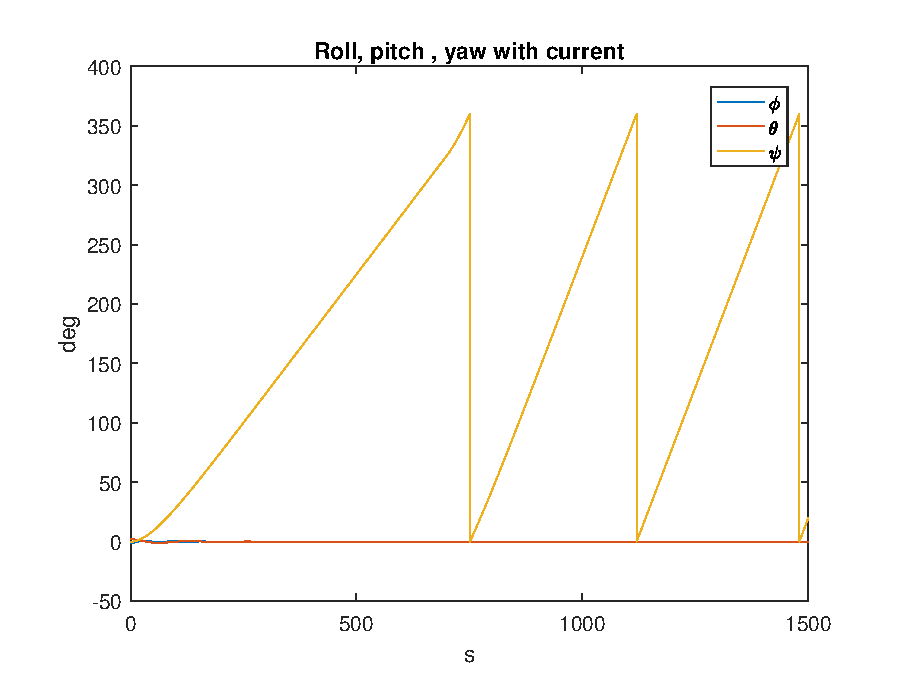
\includegraphics[width=0.6\textwidth]{figures/2_6_ang.eps}
	\caption{Plot of euler angles}
	\label{fig:2_6_ang}
\end{figure}

\begin{figure}[!ht]
	\centering
	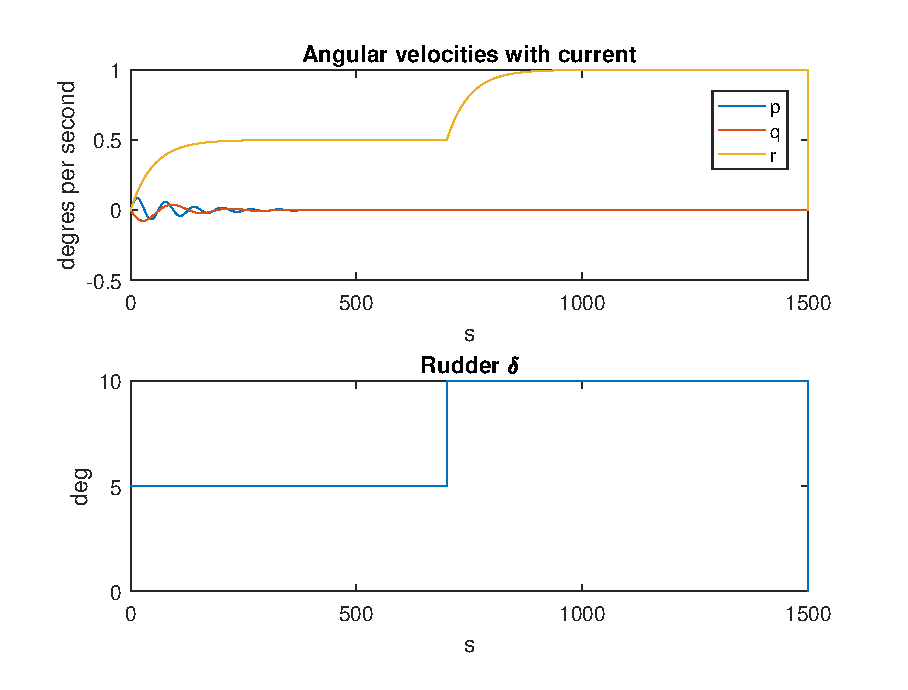
\includegraphics[width=0.6\textwidth]{figures/2_6_ang_vel.eps}
	\caption{Plot of angular velocities $\omega^b_{b/n}$}
	\label{fig:2_6_ang_vel}
\end{figure}

The plot of the position of the vehicle relative to NED in NED reference frame is represented in figure \ref{fig:2_6_pos}, both with and without current. In the plot with current, figure \ref{fig:2_6_pos_current} the shape is similar to the plot of the vehicle moving in a circle, figure \ref{fig:4_pos_current}. The difference is that this time the radius of the circles changes. This is more apparent in the position plot of the vehicle without current, figure \ref{fig:2_6_pos_without_current}. In this figure it is apparent that  in the beginning when the radius decreases, $r$ increases as it reaches its steady state. When the rudder changes at 700 seconds, it start on a "new circle" which intersects with the old bigger circle. Looking at figure \ref{fig:2_6_pos_without_current} it shows that the circle increases it's radius as time increases. This happens due to a unrealistic simplification of the model of the vehicle. When the rudder suddenly increases this simultaneously affects the velocity, from figure \figref{fig:2_6_vel} a), affecting the frequency of the signal. The result of the sudden change in frequency of the velocity is the increasing radius of the circle. Trying different switching times, different results are achieved on the form of the new circle. A switching time better matching the changing the "form" and "frequency" of the velocity, implies better matching of the frequency.  

The reason for the first circle not having increasing radius, is because the start velocity was $\mathbf{0}$, meaning there was no mismatching of frequencies.  \todo{enig alexandra ?}

Looking back at the figure representing the relative velocity of the vehicle the same discussion above also applies when the current is not zero. First the vehicle tries to drive in a bigger circle, but because of the current, the circle becomes a spiral relative to NED. It is also apparent that it takes some time after the step at 700 seconds in rudder, before the vehicle have a relative velocity such that the "circle" has a constant radius.

\begin{figure}[!ht]
	\centering
	\begin{subfigure}[b]{0.45\textwidth}
		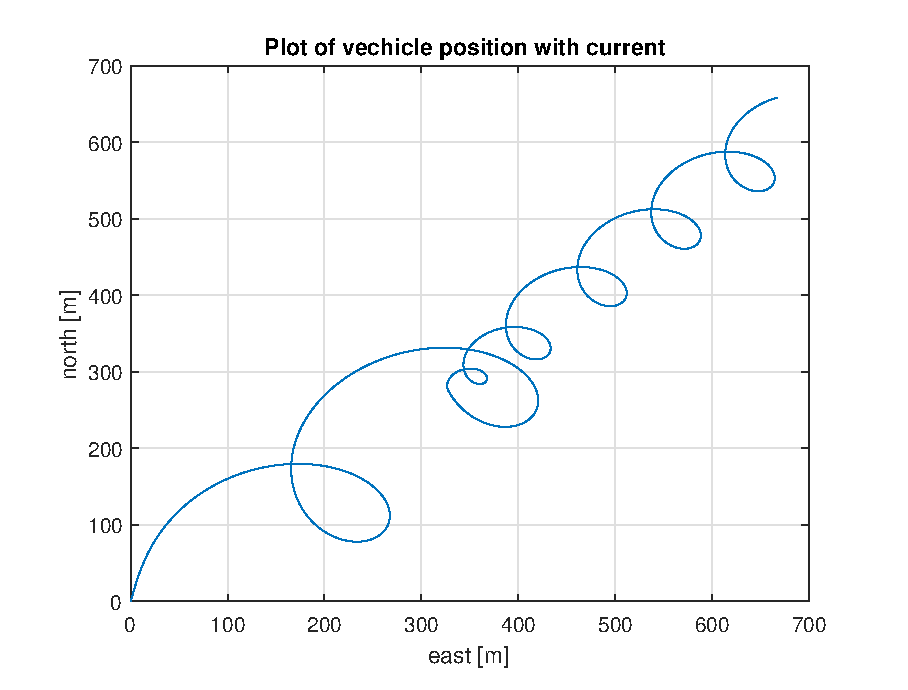
\includegraphics[width=\textwidth]{figures/2_6_pos_cur}
		\caption{Without current}
		\label{fig:2_6_pos_without_current}
	\end{subfigure}
	~ %add desired spacing between images, e. g. ~, \quad, \qquad, \hfill etc. 
	%(or a blank line to force the subfigure onto a new line)
	\begin{subfigure}[b]{0.45\textwidth}
		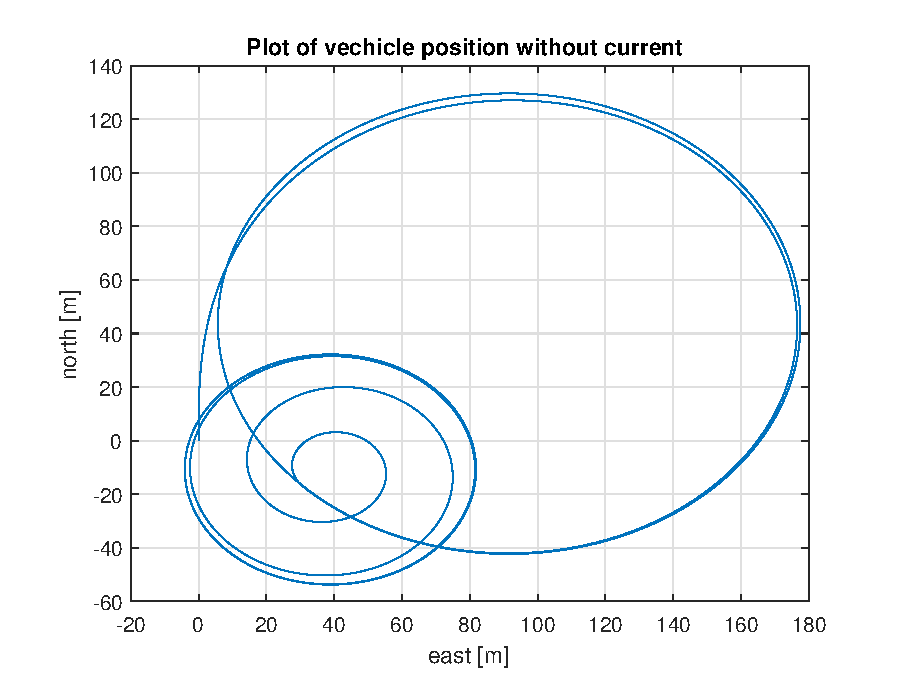
\includegraphics[width=\textwidth]{figures/2_6_pos}
		\caption{With current}
		\label{fig:2_6_pos_current}
	\end{subfigure}
	\caption{The position of the vehicle relative to NED  in reference frame NED}
	\label{fig:2_6_pos}
\end{figure}

The velocity and speed of the vehicle relative to NED and the velocity of the vehicle relative to current, both in reference frame NED is shown in figure \figref{fig:2_6_vel}. As discussed with the angular velocity $r$, this has a transient which also affects the frequency of the velocity of the vehicle. From the plot it is barley noticeable in the beginning that the periodically velocity increases the frequency of its signal. At 700 seconds, when the rudder changes, the velocities suddenly have a huge change in frequency, as discussed before. The velocity approaches a stable frequency at the same time as the rudder reaches steady state. \todo{should i discuss more about rudder ?}. Looking at the relative speed in NED vs. the relative speed to the current of the vehicle, in reference frame NED, they have similar form, but the velocity relative to NED have elevated zero compared to the velocity relative to the current, which is consistent with constant current. This is the same result as before. The speed behaves as before, with constant speed relative to current, and changing speed relative to NED. The speed relative to NED is also, of course, due to the sudden change in frequency.

\begin{figure}[!ht]
	\centering
	\begin{subfigure}[b]{0.45\textwidth}
		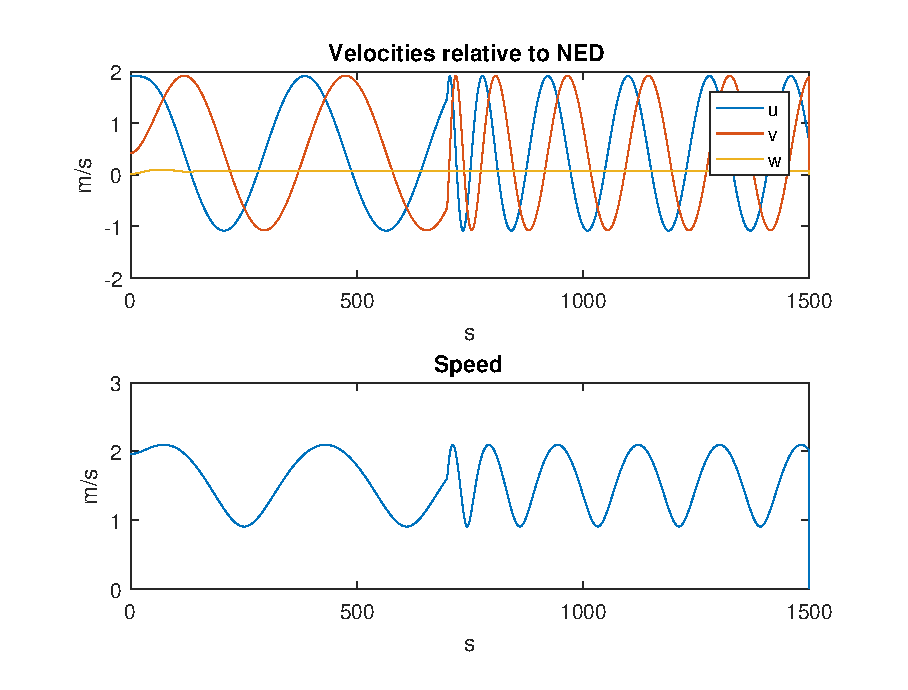
\includegraphics[width=\textwidth]{figures/2_6_vel_ned}
		\caption{Without current}
		%\label{fig:4_vel}
	\end{subfigure}
	~ %add desired spacing between images, e. g. ~, \quad, \qquad, \hfill etc. 
	%(or a blank line to force the subfigure onto a new line)
	\begin{subfigure}[b]{0.45\textwidth}
		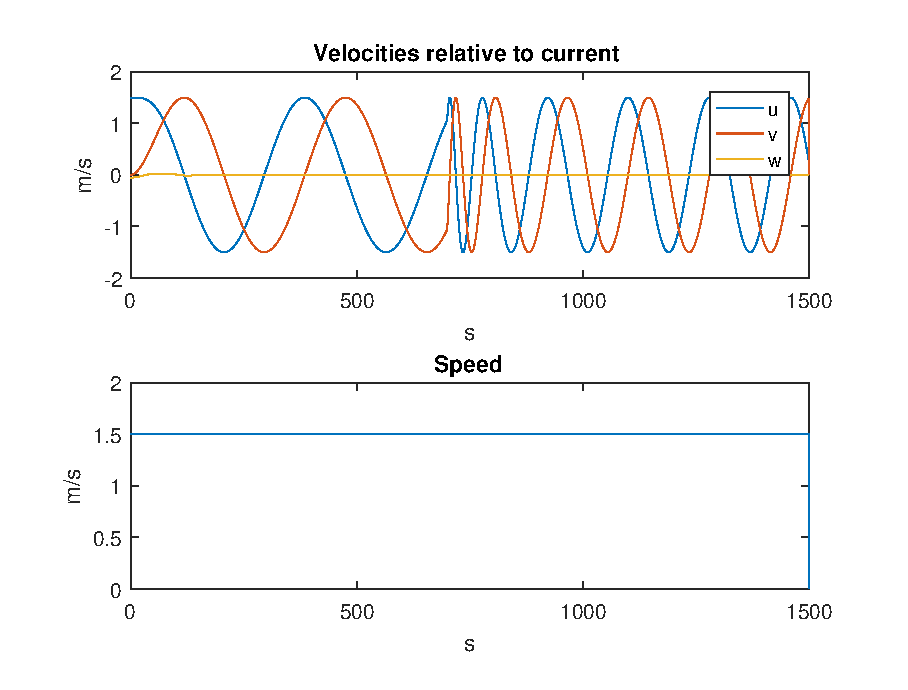
\includegraphics[width=\textwidth]{figures/2_6_vel_cur}
		\caption{With current}
		%\label{fig:4_vel_ned_with_cur}
	\end{subfigure}
	\caption{The velocity of the vehicle relative to NED  in reference frame NED}
	\label{fig:2_6_vel}
\end{figure}

The graphs of the crab angle, sideslip angle and course angle are plotted in figure \figref{fig:2_6_crab}. The figure shows that the sideslip angle increases linearly, as in problem 2.5 because it is only depending on $\mathbf{v}^b_{b/c}$. The only change in sideslip is when the frequency of the relative velocity changes, according to the change in rudder. After the change in rudder the sideslip angle have an increase in frequency (rate of going from $0 - 360 ^\circ$), which is as expected the the vehicle runs on a small circle, with same relative velocity.

As previously discussed the crab angle and the course angle depends on $\mathbf{v}^b_{b/n}$, meaning that the angle does not have linear slope. Because of the rotation of the vehicle, the yaw is not constant, as in the previous assignments. This affects the course angle so as to have to have a shorter period, going from $0-360^\circ$. The crab angle is only affected by $\mathbf{v}^n_{b/c}$ meaning it has almost the same shape as in problem 2.4 when the angular velocity $r$ is in steady state. When the $r$ is not steady state the crab angle behaves differently. The transient in the angular velocity $r$ is mostly noticeable at 700 seconds. This is because of the sudden change in rudder and mismatch of frequencies in the velocities, as discussed before. After 700 seconds, all the angles in \figref{fig:2_6_crab} have faster frequencies than before 700 s,changing from 0-360 degrees because of faster frequency in the velocity.  \todo{makes it sense to talk about frequency to angle ? }.

\begin{figure}[!ht]
	\centering
	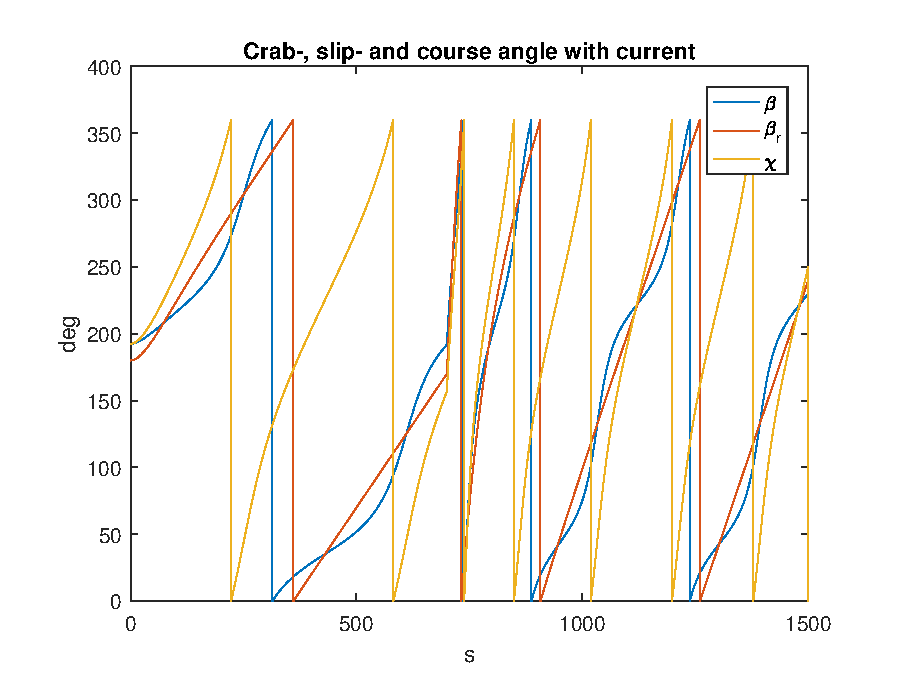
\includegraphics[width=0.6\textwidth]{figures/2_6_crab_slip_course.eps}
	\caption{Plot of the crab-, slip- and course angle}
	\label{fig:2_6_crab}
\end{figure}